% fig_circuit.tex -- edge-wise vs vertex-wise words on a length-3
% circuit; the y's rotate by one step (a 3-cycle on even positions).
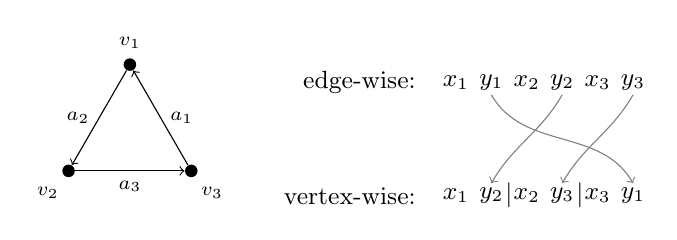
\begin{tikzpicture}[scale=0.9,
  vert/.style={circle,fill,inner sep=1.6pt},
  l/.style={inner sep=1.5pt,font=\small}]
  % the oriented triangle
  \node[vert] (v1) at (90:1) {};
  \node[vert] (v2) at (210:1) {};
  \node[vert] (v3) at (330:1) {};
  \draw[->] (v1) -- node[left,font=\scriptsize] {$a_{2}$} (v2);
  \draw[->] (v2) -- node[below,font=\scriptsize] {$a_{3}$} (v3);
  \draw[->] (v3) -- node[right,font=\scriptsize] {$a_{1}$} (v1);
  \node[font=\scriptsize,above] at (v1.north) {$v_{1}$};
  \node[font=\scriptsize,below left] at (v2.south) {$v_{2}$};
  \node[font=\scriptsize,below right] at (v3.south) {$v_{3}$};
  % the two words, one node per letter
  \begin{scope}[xshift=3.1cm,yshift=0.75cm]
    \node[l,anchor=east] at (1.0,0) {edge-wise:};
    \node[l] (ty1) at (2.0,0) {$y_{1}$};
    \node[l] (tx1) at (1.5,0) {$x_{1}$};
    \node[l] (tx2) at (2.5,0) {$x_{2}$};
    \node[l] (ty2) at (3.0,0) {$y_{2}$};
    \node[l] (tx3) at (3.5,0) {$x_{3}$};
    \node[l] (ty3) at (4.0,0) {$y_{3}$};
    \node[l,anchor=east] at (1.0,-1.6) {vertex-wise:};
    \node[l] (bx1) at (1.5,-1.6) {$x_{1}$};
    \node[l] (by2) at (2.0,-1.6) {$y_{2}$};
    \node[l] at (2.25,-1.6) {$|$};
    \node[l] (bx2) at (2.5,-1.6) {$x_{2}$};
    \node[l] (by3) at (3.0,-1.6) {$y_{3}$};
    \node[l] at (3.25,-1.6) {$|$};
    \node[l] (bx3) at (3.5,-1.6) {$x_{3}$};
    \node[l] (by1) at (4.0,-1.6) {$y_{1}$};
    \draw[->,gray] (ty1.south) to[out=-60,in=120] (by1.north);
    \draw[->,gray] (ty2.south) to[out=-120,in=60] (by2.north);
    \draw[->,gray] (ty3.south) to[out=-120,in=60] (by3.north);
  \end{scope}
\end{tikzpicture}
